%!TEX encoding = UTF-8 Unicode
% $Id: 22-nondeterminism.tex 18 2014-03-12 22:35:24Z binghe $

\chapter{非确定性}
\label{chap:nondeterminism}

程序设计语言让我们得以从烦冗的细节中脱身而出。Lisp 是一门优秀的语言,其原因
在于它本身就帮我们处理如此之多的细枝末节,同时程序员对复杂问题的容忍
是有限度的,而~Lisp 让程序员能从他们有限的耐受度中发掘出最大的潜力。

本章将会解说宏是怎么样帮助~Lisp 解决另一类重要的细节问题的:即,将非确
定性算法转换为确定性算法的问题。

本章共分为五个部分。第一部分阐述了什么是非确定性。第二部分介绍了非确定
性~\emph{choose} 和~\emph{fail} 的一个~Scheme 实现,这个实现使用
了续延。第三部分呈现
了~\emph{choose} 和~\emph{fail} 的~Common Lisp 实现,这个版本的实现
基于第~\ref{chap:continuations} 章提到的~continuation-passing 宏。第四
部分展示了如何在脱离~Prolog 的情况下,来理解~cut 操作符。最后一部分提出
了一些改进最初版本的非确定性操作符的建议。

在本章定义的非确定性选择\index{nondeterministic choice 非确定性选择}操作符,将会在第~\ref{chap:parsing_with_atns}
章里,被用来编写一个~ATN 编译器,而在第~\ref{chap:prolog} 章里,这些操
作符会被用在一个嵌入式的~Prolog 实现里面。

\section{概念}
\label{sec:nondeterminism:the_concept}

非确定性算法的运行有赖于某种超自然的预见能力。那么,既然我们没有办
法用到那种有超能力的电脑,为什么还要讨论这种算法呢?因为非确定性算法可
以用确定性的算法来\emph{模拟}。对于纯函数式程序\index{nondeterministic choice 非确定性选择!in functional programs},即那种没有副作用的程
序,要模拟非确定性简直就是小菜一碟。在纯函数式程序里面,非确定性可以用
带回溯~(backtracking) 的搜索过程来实现。

本章会展示在函数式程序里模拟非确定性的方法。如果我们有了一个能模拟非确
定性的模拟器,那么只要是真正的非确定机器能够处理的问题,照理说这个模拟
器应该也能得出答案。很多时候,写一个有超自然的洞察力助阵的程序,
肯定会比写缺乏这种能力的程序要轻松。所以如果手里能有这样一个模拟器,
写起程序来一定会如虎添翼。

%% xxx
在本节中,我们将会界定非确定性将赋予我们什么样的能力。下一节里,会用一
些示例程序展示这些能力的用处。本章开始的这两节中的例子将会使用~Scheme
编写。(Scheme 和~Common Lisp 之间的区别已经在
第~\pageref{fig:some_differences_between_scheme_and_common_lisp} 页总结
过了。)

非确定性算法和确定性算法之所以不一样,其原因在于前者能使用两种特殊的操
作符~\emph{choose}\index{choose@\emph{choose}}
和~\emph{fail}\index{fail@\emph{fail}}。\emph{Choose} 是一个函
数,它能接受一个有限的集合,并返回其中一个元素。要解释清
楚~\emph{choose} 是如何做选择的,我们必须首先介绍一下计算过程中所谓的\emph{未来}的概念。

这里,我们令~\emph{choose} 为一个函数~\texttt{choose},它接受一个列
表,并返回一个元素。对每个元素来说,如果这个元素被选中,那么这个计算过
程就会因为它而导致有一组可能的未来情况与之对应。在下列表达式中
\begin{lstlisting}
(let ((x (choose '(1 2 3))))
  (if (odd? x)
      (+ x 1)
      x))
\end{lstlisting}
接下来,当这个运算过程运行到~\texttt{choose} 这里时,将会有三个可能的
结果:
\begin{enumerate}
\item 如果~\texttt{choose} 返回~\texttt{1},那么这个运算过程将会经
  过~\texttt{if} 的~then 语句,然后返回~\texttt{2}。
\item 如果~\texttt{choose} 返回~\texttt{2},那么这个运算过程将会经
  过~\texttt{if} 的~else 语句,然后返回~\texttt{2}。
\item 如果~\texttt{choose} 返回~\texttt{3},那么这个运算过程将会经
  过~\texttt{if} 的~then 语句,然后返回~\texttt{4}。
\end{enumerate}

本例中,一旦知道~\texttt{choose} 的返回值,我们就能非常清楚这个运算
过程下一步将会是什么样子。在普遍情况下,每个选择都会和一\emph{组}将来
的情形相关联,因为在未来的某些情况下,会出现更多的选择。举个例子,如下
\begin{lstlisting}
(let ((x (choose '(2 3))))
  (if (odd? x)
      (choose '(a b))
      x))
\end{lstlisting}
在这里,在运行到第一个~\texttt{choose} 的时候,接下来会有两个可能性:
\begin{enumerate}
\item 如果~\texttt{choose} 返回~\texttt{2},那么这个运算过程将会经
  过~\texttt{if} 的~else 语句,然后返回~\texttt{2}。
\item 如果~\texttt{choose} 返回~\texttt{3},那么这个运算过程将会经
  过~\texttt{if} 的~then 语句。走到这里,运算过程到了一个岔路口,面临着
  两种可能,一个是返回~\texttt{a},另一个则返回~\texttt{b}。
\end{enumerate}

第一个集合有一个可能性,而第二个集合有两个。因而这个计算过程总共有三个可能的去向。

这里要记住的是,如果~\emph{choose} 有几个选项可供选择,那么每个选项都
会牵涉到一组可能的去向~(可能性)。\emph{Choose} 会返回哪一项呢?我们可
以像下面那样假设~\emph{choose} 的工作方式:
\begin{enumerate}
\item 如果将来的可能性中存在有情况,在这种情况下没有调
  用~\emph{fail},那么~\emph{choose} 将只会返回一个选择,
\item 如果要在零个选项里作选择,那么这个~\emph{choose} 就等价
  于~\emph{fail}。
\end{enumerate}

下面用个例子来解释,
\begin{lstlisting}
(let ((x (choose '(1 2))))
  (if (odd? x)
      (fail)
      x))
\end{lstlisting}
在上面的例子里面,每个可能的选项都有其确定的将来。既然选择~\texttt{1}
的那个选项的将来调用了~\texttt{fail},那么只有~\texttt{2} 能被选择。
所以,总的来说,这个表达式是确定性的:它总是返回~\texttt{2}。

不过,接下来的表达式就不是确定性的了:
\begin{lstlisting}
(let ((x (choose '(1 2))))
  (if (odd? x)
      (let ((y (choose '(a b))))
        (if (eq? y 'a)
            (fail)
            y))
      x))
\end{lstlisting}
第一个~\texttt{choose} 那里,有两个可能的将来与~\texttt{1} 这个选择对
应,与~\texttt{2} 对应的有一个。对于前者,这个将来是确定的,因为如果
选~\texttt{a} 的话,会导致调用~\texttt{fail}。因此,这个表达式总的来
说,要么返回~\texttt{b},要么返回~\texttt{2}。

最后一个例子,下面的表达式只有一个可能的值
\begin{lstlisting}
(let ((x (choose '(1 2))))
  (if (odd? x)
      (choose '())
      x))
\end{lstlisting}
因为,如果被选择的是~\texttt{1},那么接下来会走到一个没有待选项
的~\texttt{choose}。这个例子因而也就和上个以及另一个例子等价。
%% xxx, 为什么说:this example is thus equivalent to the last but one?

也许从上面举的几个例子,我们还不是很清楚非确定性到底意味着什么,但是我
们已经开始感受到了这种动人心魄的力量。在非确定性算法中,我们得以这样表
述~``选择一个元素,使得无论我们接下来做什么决定,都不会导致
对~\emph{fail} 调用。'' 下面的例子是一个非常典型的非确
定性算法,它能弄清楚你祖上是不是有人名叫~Igor\index{Igor}:

\begin{lstlisting}
Function Ig(n)
  if name(n) = `Igor'
     then return n
  else if parents(n)
     then return Ig(\emph{choose}(parents(n)))
  else \emph{fail}
\end{lstlisting}

\emph{fail} 操作符被用来对~\texttt{choose} 的返回值施加影响。如果我们
碰到一个~\emph{fail},那么可以推断~\emph{choose} 在此之前肯定做了错
误的选择。按照定义,\emph{choose} 的猜测总是正确的。所以,如果我们希
望确保计算过程永远不会走到一条特定的路径,那么我们所要做的就是把一
个~\emph{fail} 放到这条路径上的某个地方,那样的话,我们就不会误入歧途。
所以,由于这个算法一代一代地递归检查,函数~Ig 就能够在路径上的每一步上
作出选择,或者顺着父亲这条线索,或者顺着母亲这条线索,最终让这条路通
向~Igor。

这个过程就好像,一个程序能够这样要求:它让~\texttt{choose} 从一组选项中
找出某个元素,只要需要的话,就使用~\texttt{choose} 的返回值作为判断的依
据,只要~\emph{fail} 出现,就一票否决,用这个机制倒推出程序希
望~\emph{choose} 在此之前作出的选择。接着,一眨眼功
夫,\emph{choose} 的返回值就是我们想要的结果。在这个模型
中,\emph{choose} 体现出了它预知未来的能力\index{nondeterministic choice 非确定性选择!appearance of foresight 预知未来的表象}。

实际上,\emph{choose} 并没有什么超自然的神力。\emph{choose} 的任意
一个实现都必须能通过在发现错误的时候进行回溯,来模拟准确无误的猜测,这
个过程就像小老鼠能在迷宫里找到出路一样。但是回溯可以不动声色地发生于
无形之间。一旦你有某种形式的~\emph{choose} 和~\emph{fail},就可以
写出像上面例子那样的算法了,感觉就像这个算法真的知道应该选择哪一个祖先一
样。借助~\emph{choose},只要写一个遍历问题空间的算法,就能搜索这个问
题空间了。

\section{搜索}
\label{sec:nondeterminism:search}
\index{nondeterministic choice 非确定性选择!and search}

有许多经典的问题都可以归结为搜索问题,对于这类问题,非确定性常常被证明
是一种行之有效的抽象方式。假设~\verb|nodes| 被绑定到一棵树上节点组成
的列表,而~\texttt{(kids $n$)} 是一个能返回节点~\emph{n} 的子节
点的函数,如果~\emph{n} 没有子节点的话,就返回~\texttt{\#f}。我们打算写一
个函数,即~\texttt{(descent $n_1$ $n_2$)},让它返回从节点~$n_1$ 到其子
孙节点~$n_2$~(如果有的话) 所经过的某条路径上所有节点构成的列表。
图~\ref{fig:deterministic_tree_search} 中就是这个函数的一个确定性版本。
\begin{figure}
\begin{lstlisting}
(define (descent n1 n2)
  (if (eq? n1 n2)
      (list n2)
      (let ((p (try-paths (kids n1) n2)))
         (if p (cons n1 p) #f))))

(define (try-paths ns n2)
  (if (null? ns)
      #f
      (or (descent (car ns) n2)
           (try-paths (cdr ns) n2))))
\end{lstlisting}
\caption{确定性的树搜索}
\label{fig:deterministic_tree_search}
\end{figure}

非确定性让程序员不用再操心路径寻找的细节。而只要告
诉~\texttt{choose},让它找到一个节点~$n$,使得从~$n$ 到我们的目标节点存
在一条路径。用非确定性的办法,我们可以写出更简单的~\texttt{descent} 版
本,如图~\ref{fig:nondeterministic_tree_search} 所示。

图~\ref{fig:nondeterministic_tree_search} 中的版本并没有显式地去搜索正
确的路径所在的节点。能这样写,是基于这样的假设:即~\texttt{choose} 已经
找到了一个具有期望特性的~\texttt{n}。如果我们习惯于阅读确定性的程序,可
能就很难认识到这一点,即:\texttt{choose} 毫无疑问是能完成工作的,就好
像它能\emph{猜出来}到底是哪个~\texttt{n} 能让自己指引整个计算过程一帆
风顺、正确无误~(fail) 地走到终点。

\begin{figure}
\begin{lstlisting}
(define (descent n1 n2)
  (cond ((eq? n1 n2) (list n2))
        ((null? (kids n1)) (fail))
        (else (cons n1 (descent (choose (kids n1)) n2)))))
\end{lstlisting}
\caption{非确定性的树搜索}
\label{fig:nondeterministic_tree_search}
\end{figure}

对于~\emph{choose} 的能力,大概更有说服力的实例要算:即使在函数调用的
时候,它的预见力也能奏效。图~\ref{fig:choice_in_a_subroutine} 里有一对
函数,它们能猜出两个数字,让两个数字之和等于调用者给出的数字。在第一个
函数~\texttt{two-numbers} 里面,非确定性帮助选择出两个数字,并把它们作
为一个列表返回。当我们调用~\texttt{parlor-trick} 的时候,它会通过调
用~\texttt{two-numbers} 来得到这两个数字。请注
意,在~\texttt{two-numbers} 在做决定的时候,它根本就无从得知用户给出的
那个数字到底是多少。

\begin{figure}
\begin{lstlisting}
(define (two-numbers)
  (list (choose '(0 1 2 3 4 5))
        (choose '(0 1 2 3 4 5))))

(define (parlor-trick sum)
  (let ((nums (two-numbers)))
    (if (= (apply + nums) sum)
        `(the sum of ,@nums)
        (fail))))
\end{lstlisting}
\caption{在子函数里的选择非确定性的树搜索}
\label{fig:choice_in_a_subroutine}
\end{figure}


要是~\texttt{choose} 猜的两个数字加起来不等于用户输入的数字,那么这个计
算过程会以失败告终。由于我们可以信赖~\texttt{choose},相信只要存在路径
不通向失败的话,\texttt{choose} 选择的路径上就不会有失败存在。因此我
们才能假定一旦调用方给出的数字在合适的区间内,\texttt{choose} 就肯定
会作出正确的猜测,实际上它就是能做到这一点:\footnote{由于~Scheme 没有
  指定参数求值的顺序~(正相反,Common Lisp 要求求值的顺序为从左至右),这
  次调用也可能会返回~\texttt{(THE SUM OF 5 2)}。}
\begin{lstlisting}
> (parlor-trick 7)
(THE SUM OF 2 5)
\end{lstlisting}

在简单的搜索问题中,Common Lisp 内置的~\texttt{find-if} 函数一样能完成
任务。那么非确定性选择到底有什么优越性呢?为什么不在待选项的列表里面一
个一个找过来,搜索那些具有期望特性的元素呢?\index{iteration!vs. nondeterministic choice}\index{nondeterministic choice 非确定性选择!vs. iteration}\emph{choose} 和传统的迭代
搜索最根本的区别在于:\emph{choose} 对于\emph{失败} 到底能看到多
远\index{choose@\emph{choose}!extend of 止境}是没有止境的。非确定
性~\emph{choose} 可以知道未来任意远的事情。如果将来在某一点会发生导
致~\emph{choose} 做出无效选择的事件,我们可以确信~\emph{choose} 自
己知道如何避免作出这样猜测。正如我们在~\texttt{parlor-trick} 一例中所见
到的,甚至在我们从~\emph{choose}发生的函数中返回之后,\emph{fail}
操作符仍然能正常工作。

举例来说,这种失败机制常发生在~Prolog 进行的搜索中,非确定性之所以
在~Prolog 里能大显神通的原因在于,这门语言的一个核心特性是它能每次只返回
所有查询结果中的一个。倘若使用非确定性的方法,而不是一次返回所有的有
效结果,Prolog 就有能力处理递归的规则和条件,否则它就会得出一个大小为无
穷大的结果集合。

看到~\texttt{descent} 的第一反应,可能就和看到归并排序算法的第一反应差
不多:它到底是在哪里完成的工作的呢?就像归并排序一样,工作是在不知不觉中
完成的,但是的确是完成了。第~\ref{sec:scheme_implementation} 节会介绍一
个~\emph{choose} 实现,迄今为止在这个实现里,所有的代码示例都是实际使
用的程序。

这些例子体现了非确定性作为一种抽象手段的价值所在。最优秀的编程语言抽象
手段不仅仅是让你省下了打字的时间,更重要的是让你更省心。在自动机理论
\index{automata theory 自动机理论}里面,要是没有非确定性的话,有些证明
简直就难以想象,无法完成。一门允许非确定性的语言也能给程序员创造类似的
有利条件。

\section{Scheme 实现}
\label{sec:scheme_implementation}
这一节将会解释续延~(continuation) 是如何模拟非确定性的。
图~\ref{fig:scheme_implementation_of_choose_and_fail} 
是~\emph{choose} 和~\emph{fail} 的~Scheme 实现\note{292}。在表象之
下,\texttt{choose} 和~\texttt{fail} 利用回溯\index{backtracking}来模拟非确定性。然
而,一个使用回溯的搜索程序必须保留足够的信息才能在先前选中的选择失
败后,继续使用其他的选项搜索。这些信息就以续延的形式保存在全局变
量~\texttt{*paths*} 里面。

\begin{figure}
\begin{lstlisting}
(define *paths* ())
(define failsym '@)

(define (choose choices)
  (if (null? choices)
      (fail)
      (call-with-current-continuation
        (lambda (cc)
          (set! *paths*
                (cons (lambda ()
                        (cc (choose (cdr choices))))
                      *paths*))
          (car choices)))))

(define fail)

(call-with-current-continuation
  (lambda (cc)
    (set! fail
          (lambda ()
            (if (null? *paths*)
                (cc failsym)
                (let ((p1 (car *paths*)))
                  (set! *paths* (cdr *paths*))
                  (p1)))))))
\end{lstlisting}
\caption{\emph{choose} 和~\emph{fail} 的~Scheme 实现}
\label{fig:scheme_implementation_of_choose_and_fail}
\index{nondeterministic choice 非确定性选择!Scheme implementation Scheme 实现}
\index{choose@\texttt{choose}!Scheme version}
\index{fail@\texttt{fail}!Scheme version}
\end{figure}

传给函数~\texttt{choose} 的是一个名为~\texttt{choices} 的列表,它由一系
列选项构成。如果~\texttt{choice} 是空的,那么~\texttt{choose} 就会调
用~\texttt{fail},后者会把计算过程打回之前的~\texttt{choose}。如
果~\texttt{choices} 是~\texttt{($first$ . $rest$)} 的形式,那
么~\texttt{choose} 会首先把它调用~$rest$ 时的续延压
入~\texttt{*paths*},然后再返回~$first$。

相比之下,函数~\texttt{fail} 就简单一些。它直接从~\texttt{*paths*} 弹出
一个续延,然后调用它。如果之前保存的路径都被用完了,\texttt{fail}就返回
符号~\texttt{@}。不过,它不会简简单单地像普通的函数返回值那样返回这个符
号,也不会把它作为最近的一次~\texttt{choose} 的返回值来返回。我们真正想
要做的是把~\texttt{@} 直接返回到~toplevel
\index{call-with-current-continuation (call/cc)@\texttt{call-with-current-continuation} (\texttt{call/cc})!at toplevel} 。这个目的是这样达到的:通过
把~\texttt{cc} 绑定到定义~\texttt{fail} 时所处的那个续延,而定
义~\texttt{fail} 的地方可以被认为是~toplevel。通过调用~\texttt{cc},
\texttt{fail} 可以直接返回到那里。


图~\ref{fig:scheme_implementation_of_choose_and_fail} 的实现
把~\texttt{*paths*} 当成栈来用。在这个实现里面,每当失败的时候就会转而
从最新近的抉择点重新开始。这种策略被称为\emph{按时间回
  溯~(chrnonological backtracking)}\index{chrnonological backtracking},
其结果就是在问题空间中的深度优先\index{nondeterministic choice 非确定性选择!depth-first 深度优先}
搜索。``非确定性''这个词常会被滥用,就
好像它是深度优先实现的代名词。Floyd\index{Floyd, Robert W.} 关
于非确定性算法的那篇经典的论文中提到的术语``非确定性'',取的就是这个意思
\note{293},而且我们看到的一些非确定性解析器~(parser) 和~Prolog 里面,
非确定性算法的实现都是用的深度优先搜索。\index{recursion 递归!in grammars}不过,也要注意到,
图~\ref{fig:scheme_implementation_of_choose_and_fail} 并非唯一的实现,
甚至算不上一个正确的实现。照道理来说,~\emph{choose} 应该能根据任意可
计算的指标来选择对象。但是,如果一个图里面有环的话,程序使用这些版本
的~\texttt{choose} 和~\texttt{fail} 来搜索这个图就无法终止了\index{nondeterministic choice 非确定性选择!depth-first 深度优先!nonterminating}。

在实际应用中,非确定性常常意味着使用和
图~\ref{fig:scheme_implementation_of_choose_and_fail} 中等价的的深度优
先实现,同时把避免在搜索空间里面绕圈子的问题留给用户去解决。不过,对这一主题
有兴趣的读者,在本章的最后一节将会解释如何实现真正的~\emph{choose}
和~\emph{fail}。

\section{Common Lisp 实现}
\label{sec:common_lisp_implementation}

这一节将阐述如何用~Common Lisp 来实现~\emph{choose} 和~\emph{fail}
一种表现形式。正如我们在上节所看到的,\texttt{call/cc} 使得在~Scheme 里
面能轻而易举地实现非确定性机制。之前,我们对计算过程的未来定义了一个理
论中的概念,续延把它给具体化了。在~Common Lisp 中,我们可以用在
第~\ref{chap:continuations} 章中给出的~continuation-passing 宏\index{continuation-passing macros!use in nondeterministic choice}来实现它。
借助这些宏,我们就能给出仅仅比上一节中的~Scheme 版本稍微难看一些
的~\emph{choose},但是它们在实际使用中的效果是一样的。

\begin{figure}
\begin{lstlisting}
(defparameter *paths* nil)
(defconstant failsym '@)

(defmacro choose (&rest choices)
  (if choices
      `(progn
         ,@(mapcar #'(lambda (c)
                       `(push #'(lambda () ,c) *paths*))
                   (reverse (cdr choices)))
         ,(car choices))
      '(fail)))

(defmacro choose-bind (var choices &body body)
  `(cb #'(lambda (,var) ,@body) ,choices))

(defun cb (fn choices)
  (if choices
     (progn
       (if (cdr choices)
           (push #'(lambda () (cb fn (cdr choices)))
                 *paths*))
       (funcall fn (car choices)))
     (fail)))

(defun fail ()
  (if *paths*
      (funcall (pop *paths*))
      failsym))
\end{lstlisting}
\caption{非确定性操作符的~Common Lisp 实现}
\label{fig:nondeterministic_operators_in_common_lisp}
\index{choose@\texttt{choose}!Common Lisp version}
\index{choose-bind@\texttt{choose-bind}}
\index{fail@\texttt{fail}!Common Lisp version}
\index{nondeterministic choice 非确定性选择!Common Lisp implementation Common Lisp 实现}
\end{figure}

图~\ref{fig:nondeterministic_operators_in_common_lisp} 中是一
个~\emph{fail} 的~Common Lisp 实现,以及两个版本的~\emph{choose}。
其中一个~\emph{choose} 的~Common Lisp 版本和它的~Scheme 版本有些微小
的区别。Scheme 的~\emph{choose} 接受一个参数,即:一个待选项的列
表,以备选择作为返回值。而~Common Lisp 版本采用了~\texttt{progn} 的语法。
它后面可以跟任意多个表达式,\emph{choose} 会从里面选出一个进行求值:
\begin{lstlisting}
> (defun do2 (x)
    (choose (+ x 2) (* x 2) (expt x 2)))
DO2
> (do2 3)
5
> (fail)
6
\end{lstlisting}

在~toplevel,我们可以把回溯算法看得更清楚一些,它运行在非确定性搜索的幕
后。变量~\texttt{*paths*} 被用来保存还没有走过的路径。当计算过程到达一
个有多个可选项的~\texttt{choose} 表达式的时候,第一个可选项会被求值,而
其它几个选项则会被保存在~\texttt{*paths*} 里。如果程序在这之后碰到
了~\texttt{fail},那么最后一个被保存的选项会从~\texttt{*paths*} 弹出来,
然后重新开始计算。要是没有更多的路径可供重启计算的话,\texttt{fail} 会
返回一个特殊的值\index{"@@\texttt{"@}}:
\begin{lstlisting}
> (fail)
9
> (fail)
@
\end{lstlisting}

在图~\ref{fig:nondeterministic_operators_in_common_lisp} 中,用来表示
失败的常量~\texttt{failsym},被定义成了符号~\texttt{@}。如果你希望
把~\texttt{@} 作为一个普通的返回值,那么可以把~\texttt{failsym} 改成
用~gensym。

另一个非确定性的选择操作符~\texttt{choose-bind} 的实现用了一个稍微不一
样的形式。它接受的是一个符号、一个待选项的列表,还有一个代码体。
\texttt{choose-bind} 会对这个待选项的列表运行~\emph{choose},然后把被
选中的值绑定到符号上,最后对代码体求值:
\begin{lstlisting}
> (choose-bind x '(marrakesh strasbourg vegas)
    (format nil "Let's go to ~A." x))
"Let's go to MARRAKESH."
> (fail)
"Let's go to STRASBOURG."
\end{lstlisting}

Common Lisp 的实现中提供两个选择操作符的原因只是为了方便。你可以
用~\texttt{choose-bind} 达到和~\texttt{choose} 一样的效果,只要把:
\begin{lstlisting}
(choose (foo) (bar))
\end{lstlisting}
翻译成
\begin{lstlisting}
(choose-bind x '(1 2)
 (case x
   (1 (foo))
   (2 (bar))))
\end{lstlisting}
就可以了。但是如果在这个情况下我们有一个单独的操作符的话,程序的可读性
就会更好些。\footnote{如果需要的话,对外的接口可以只提供单独一个操作
  符,因为~\texttt{(fail)} 和~\texttt{(choose)} 是等价的。}

Common Lisp 的选择操作符通过闭包\index{functions 函数!closures of!use in nondeterministic choice}和变量捕捉保存了几个相关变量的绑
定。\texttt{choose} 和~\texttt{choose-bind} 作为宏,在它们所在的表达式
的词法环境中展开。注意到,这两个宏加入~\texttt{*paths*} 的是一个闭
包,在这个闭包保存了将要用到的待选项,还有被引用到的词法变量的所有绑
定。举例来说,在下面的表达式里
\begin{lstlisting}
(let ((x 2))
  (choose
    (+ x 1)
    (+ x 100)))
\end{lstlisting}

当启用之前保存的选项重新开始计算时,就会用到~\texttt{x}。这就是为什么
让~\texttt{choose} 把它的参数包装在一个~lambda 表达式的原因所在。上面的
表达式展开后的结果如下:
\begin{lstlisting}
(let ((x 2))
  (progn
    (push #'(lambda () (+ x 100))
          *paths*)
    (+ x 1)))
\end{lstlisting}

保存在~\texttt{*path*} 上的对象是一个含有指向~\texttt{x} 指针的闭包。这
是由于要闭包里存放变量的需要使然,可以从这一点看出~Scheme 和~Common
Lisp 两者的选择操作符在语义上的不同之处。

倘若我们把~\texttt{choose} 和~\texttt{fail} 和
第~\ref{chap:continuations} 章的~continuation-passing 宏一起用,那么指
向我们的续延变量~\texttt{*cont*} 的一个指针也会一样被保存下来。如果
用~\texttt{=defun} 来定义函数,同时用~\texttt{=bind} 来调用它们,而且
用~\texttt{=values} 来获取函数的返回值,我们就可以在任意一个~Common
Lisp 程序里使用这套非确定性的机制了。
\index{nondeterministic choice 非确定性选择!Common Lisp implementation Common Lisp 实现!need for CPS macros CPS 宏的要求}

\begin{figure}
\begin{lstlisting}
(=defun two-numbers ()
  (choose-bind n1 '(0 1 2 3 4 5)
    (choose-bind n2 '(0 1 2 3 4 5)
      (=values n1 n2))))
(=defun parlor-trick (sum)
  (=bind (n1 n2) (two-numbers)
    (if (= (+ n1 n2) sum)
        `(the sum of ,n1 ,n2)
        (fail))))
\end{lstlisting}
\caption{Common Lisp 版的``在子函数里作选择''}
\label{fig:common_lisp_choice_in_a_subroutine}
\end{figure}

在这些宏的帮助下,我们可以毫无问题地运行那个非确定性的选择发生在子函数
里的那个例子了。图~\ref{fig:common_lisp_choice_in_a_subroutine} 中展示
了~Common Lisp 版本的~\texttt{parlor-trick},就像之前它在~Scheme 里一
样,它运行正常:
\begin{lstlisting}
> (parlor-trick 7)
(THE SUM OF 2 5)
\end{lstlisting}

这个函数之所以能正常工作,是因为表达式
\begin{lstlisting}
(=values n1 n2)
\end{lstlisting}

在两个~\texttt{choose-bind} 中被展开成了
\begin{lstlisting}
(funcall *cont* n1 n2)
\end{lstlisting}
而每个~\texttt{choose-bind} 则都被展开成了一个闭包,每个闭包都保存有指
向~body 中引用过的变量的指针,这些变量中包括~\texttt{*cont*}。

在使用~\texttt{choose}、\texttt{choose-bind} 和~\texttt{fail} 过程中存
在的种种限制和图~\ref{fig:restrictions_on_continuation-passing_macros} 中所
展示的限制是一样的\index{nondeterministic choice 非确定性选择!Common Lisp implementation Common Lisp 实现!restrictions on 其限制},后者代码中所使用的技术是~continuation-passing 宏。
只要是选择表达式,它就一定是最后一个被求值的。所以如果我们想要在~Common
Lisp 里做一系列的选择的话,这些选择就必须以嵌套的形式出现:

\begin{lstlisting}
> (choose-bind first-name '(henry william)
    (choose-bind last-name '(james higgins)
      (=values (list first-name last-name))))
(HENRY JAMES)
> (fail)
(HENRY HIGGINS)
> (fail)
(WILLIAM JAMES)
\end{lstlisting}
和平时一样,这样做的结果就是深度优先搜索。

在第~\ref{chap:continuations} 章定义的操作符能让表达式享有最后求值的权利。
这个权利由新的宏抽象层接管了,一个~\texttt{=values} 表达式必须出现在~\texttt{choose} 表达式里面,反过来就行不通。也就是说
\begin{lstlisting}
(choose (=values 1) (=values 2))
\end{lstlisting}
是可以的,但是
\begin{lstlisting}[escapechar=\@]
(=values (choose 1 2))        @\hfill@; wrong
\end{lstlisting}
却不行。(在后面的例子中,\texttt{choose} 的展开式是无法
在~\texttt{=values} 的展开式里捕获~\texttt{*cont*} 的变量实例的。)

只要我们注意不要超越这里列出的以及
图~\ref{fig:restrictions_on_continuation-passing_macros} 所示的那些限
制,Common Lisp 的非确定选择机制就将会和它在~Scheme 中一样,正常工作。
与图~\ref{fig:nondeterministic_tree_search} 中的~Scheme 版的非确定性树
搜索算法相对应,图~\ref{fig:nondeterministic_search_in_common_lisp} 中
所示的是它的~Common Lisp 版本。Common Lisp 版的~\texttt{descent} 是从它
的~Scheme 版本直译过来的,尽管它显得有点罗嗦,同时也没那么漂亮。

\begin{figure}
\begin{lstlisting}
> (=defun descent (n1 n2)
    (cond ((eq n1 n2) (=values (list n2)))
          ((kids n1) (choose-bind n (kids n1)
                       (=bind (p) (descent n n2)
                          (=values (cons n1 p)))))
          (t (fail))))
DESCENT
> (defun kids (n)
    (case n
      (a '(b c))
      (b '(d e))
      (c '(d f))
      (f '(g))))
KIDS
> (descent 'a 'g)
(A C F G)
> (fail)
@
> (descent 'a 'd)
(A B D)
> (fail)
(A C D)
> (fail)
@
> (descent 'a 'h)
@
\end{lstlisting}
\caption{在~Common Lisp 里做非确定性搜索}
\label{fig:nondeterministic_search_in_common_lisp}
\end{figure}

现在有了~Common Lisp 版的\utility,就能做非确定性的搜索,而不用显式
地去做回溯了。虽然劳心费力写了这些代码,但可以从此把本会写得冗长拖
沓、一团乱麻的代码用寥寥几行就说得清楚明白,这个回报还是值得的。在现有
的宏基础上再构造另一层宏,我们就能够用一页纸的篇幅写出一个~ATN 编译
器~(第~\ref{chap:parsing_with_atns} 章),或是在两页纸上初步实
现~Prolog~(第~\ref{chap:prolog} 章)。

使用了~\texttt{choose} 的~Common Lisp 程序在编译的时候必须打开尾递归优化
  \index{nondeterministic choice 非确定性选择!Common Lisp implementation Common Lisp 实现!and tail-recursion optimization 以及尾递归优化}
  \index{continuation-passing macros!and tail-recursion optimization}
  \index{tail-recursion optimization 尾递归优化!needed with CPS macros}
  \index{nondeterministic choice 非确定性选择!optimizing},
这不只是为了加快程序的运行速度,更重要的是为了避免
发生栈溢出。虽然程序是通过调用续延函数来``返回''值的,但是它真正的返回
却是等碰到了最后的~\texttt{fail} 才发生的。要是不进行尾递归优化,程序占
用的栈空间只会越来越大。\note{298}

\section{减枝}
\label{sec:cuts}
\index{cut!in Lisp}

本节将会告诉我们如何在进行非确定性选择的~Scheme 程序里使用减枝~(cut)。虽
然~cut 一词来自于~Prolog,但是对非确定性来说,它所代表的概念却是普适的。
你可以在任意一个作非确定性选择的程序里使用减枝技术。

如果不把~Prolog 牵扯进来,可以更容易地理解减枝。让我们先设想一个现实生
活中的例子。假设花生糖\index{Chocoblob 花生糖}\footnote{译者注:原文为~``Chocoblob'',
是一种巧克力糖。但为了更通顺,译者自作主张把它改为~``花生糖''。}
的生产厂商决定进行一次促销活动。出厂时,一小部分的花生糖盒子
里会装有可以用来领奖的兑奖币。为了确保公平,发货的时候不会同时把两个有
奖品的盒子送往一个城市。

促销开始后,糖厂发现由于兑奖币太小了,很容易被小孩误吞下去。这个发现
让糖厂的律师\index{lawyers 律师}预见到了由此导致的索赔和诉讼,别无他法,他们只得发起紧
急搜索,想要召回全部有奖的盒子。每个城市都有多家门店销售花生糖,而每个
店都会有不止一个盒子。但是律师们用不着打开每一个包装盒,因为
只要他们一旦在某个城市发现有硬币的盒子,就不用再在这个城市里检查其他盒
子了,因为每个城市最多只有一个有奖的盒子。要实现这个算法,可以做个减枝操作。

\emph{减枝} 指的是排除搜索树里的一部分。对于花生糖问题来说,搜索树是实
实在在存在的:根节点是公司的总部,这个节点的子节点是奖盒所发往的城
市,而这些子节点的子节点则是每个城市里面的门店,每个门店的子节点则代表
了相应门店里的包装盒。当律师们搜索这棵树时,如果找到了有硬币的盒子
时,他们会裁减掉当前城市下,还未检查过的分支。

减枝操作实际上含有两个步骤:当你知道那一部分的搜索树已经没有价值了,你
就可以进行一次减枝,但是首先你必须在树上你认为可以减枝的地方作上标记。
在花生糖的例子里,我们从常识可以推知,我们一搜索到城市的时候,这棵树
的标记就做好了。很难用抽象的术语说清楚~Prolog 的~cut 是干什么的,因为这
种标记是隐式的。不过用显式的标记操作符的话,减枝的意思就比较容易理解了。

\begin{figure}
\begin{lstlisting}
(define (find-boxes)
  (set! *paths* ())
  (let ((city (choose '(la ny bos))))
    (newline)
    (let* ((store (choose '(1 2)))
           (box (choose '(1 2))))
      (let ((triple (list city store box)))
        (display triple)
        (if (coin? triple)
            (display 'c))
        (fail)))))

(define (coin? x)
  (member x '((la 1 2) (ny 1 1) (bos 2 2))))
\end{lstlisting}
\caption{穷尽的花生糖搜索}
\label{fig:exhaustive_chocoblob_search}
\end{figure}

图~\ref{fig:exhaustive_chocoblob_search} 中的程序用非确定性的方法搜索了一
个规模更小的花生糖树。每当一个盒子被打开,程序就会显示一个~($city$
$store$ $box$) 的列表。如果盒子里面有硬币的话,在其后会再打印一个~\texttt{c}:
\begin{lstlisting}
> (find-boxes)
(LA 1 1)(LA 1 2)C(LA 2 1)(LA 2 2)
(NY 1 1)C(NY 1 2)(NY 2 1)(NY 2 2)
(BOS 1 1)(BOS 1 2)(BOS 2 1)(BOS 2 2)C
@
\end{lstlisting}

要实现花生糖的律师们想出的优化搜索算法,我们需要两个新的操作
符:\texttt{mark} 和~\texttt{cut}。
图~\ref{fig:marking_and_pruning_search_trees} 展示了一种定义它们
的方法。虽然非确定性本身和特定的实现没什么关系,我们可以通过任意一个实
现来理解它,但是搜索树的剪枝作为一种优化技术却高度依赖
~\texttt{choose} 的实现细节。
图~\ref{fig:marking_and_pruning_search_trees} 中所示
的~\texttt{mark} 和~\texttt{cut} 适用于深度优先搜索类
型~\texttt{choose} 实现~(图~\ref{fig:scheme_implementation_of_choose_and_fail})。

%% binghe: change equal? to eq? according to orignal errata
\begin{figure}
\begin{lstlisting}
(define (mark) (set! *paths* (cons fail *paths*)))

(define (cut)
  (cond ((null? *paths*))
        ((eq? (car *paths*) fail)
         (set! *paths* (cdr *paths*)))
        (else
         (set! *paths* (cdr *paths*))
         (cut))))
\end{lstlisting}
\caption{对搜索树进行标记和剪枝}
\label{fig:marking_and_pruning_search_trees}
\index{cut@\texttt{cut}}
\index{mark@\texttt{mark}}
\end{figure}

要做~\texttt{mark},通常的思路是把标记存到~\texttt{*paths*} 里,后者是
个列表,被用来保存还没有检查过的选择点。调用~\texttt{cut} 会
让~\texttt{*paths*} 一直退栈,直到弹出最新近压入的标记。但是,我们应该
把什么作为标记呢?我们有几个选择,比如说,也许我们可以用符
号~\texttt{m},但是这样的话,我们就需要重写~\texttt{fail},让它在碰
到~\texttt{m} 的时候忽略它。幸亏函数也是一种对象,至少还有一种标记让我
们能用~\texttt{fail},它就是:函数~\texttt{fail} 本身。这样的话,如
果在一个标记上发生了~\texttt{fail},让它调用自己就可以了。

\begin{figure}
\begin{lstlisting}[escapechar=\@]
(define (find-boxes)
  (set! *paths* ())
  (let ((city (choose '(la ny bos))))
    (mark)                                  @\hfill@;
    (newline)
    (let* ((store (choose '(1 2)))
           (box (choose '(1 2))))
      (let ((triple (list city store box)))
        (display triple)
        (if (coin? triple)
            (begin (cut) (display 'c)))     @\hfill@;
        (fail)))))
              Figure 22.10: 
\end{lstlisting}
\caption{剪枝的花生糖搜索}
\label{fig:pruned_chocoblob_search}
\end{figure}

图~\ref{fig:pruned_chocoblob_search} 中显示了如何使用这些操作符来对
花生糖的例子中的搜索树进行剪枝。(被修改过代码所在的行被用分号注明) 每当选
择一个城市的时候,我们都会调用~\texttt{mark} 。在那
时,\texttt{*paths*} 里有一个续延,它保存着对剩余城市的搜索状态。

如果我们找到一个有硬币的盒子,就调用~\texttt{cut},它会
让~\texttt{*path*} 恢复到之前做标记的状态。执行减枝的效果直到下次调
用~\texttt{fail} 的时候才能看出来。但是到了那个时
候,在~\texttt{display} 之后,下一个~\texttt{fail} 会把搜索过程直接带到
最外层的~\texttt{choose} 那里,就算在搜索树中更下层的地方还有一些没有碰
过的选择点,也是这样。结果就是:一旦找到了有硬币的盒子,我们就会从
下一个城市继续我们的搜索,如下:

\begin{lstlisting}
> (find-boxes)
(LA 1 1)(LA 1 2)C
(NY 1 1)C
(BOS 1 1)(BOS 1 2)(BOS 2 1)(BOS 2 2)C
@
\end{lstlisting}
在本例中,我们只检查了七个盒子,而不是十二个。

\section{真正的非确定性}
\label{sec:true_nondeterminism}

确定性的图搜索程序应该采取专门的措施,以免在循环路径上无法脱身。
图~\ref{fig:a_directed_graph_with_a_loop} 中所示是一个包含环路的有向图。
当程序在一条从节点~\texttt{a} 通向节点~\texttt{e} 的路径上搜索时,就有
可能陷入由~$\langle$\texttt{a}, \texttt{b}, \texttt{c}$\rangle$ 构成的
环状路径。除非这个确定性搜索使用了随机算法,广度优先搜索,或者显式地检
测循环路径,否则是无法避免死循环的。如
图~\ref{fig:deterministic_search} 所示,是~\texttt{path} 的实现,其中使
用了广度优先搜索,避免了环路。

\begin{figure}
\begin{center}
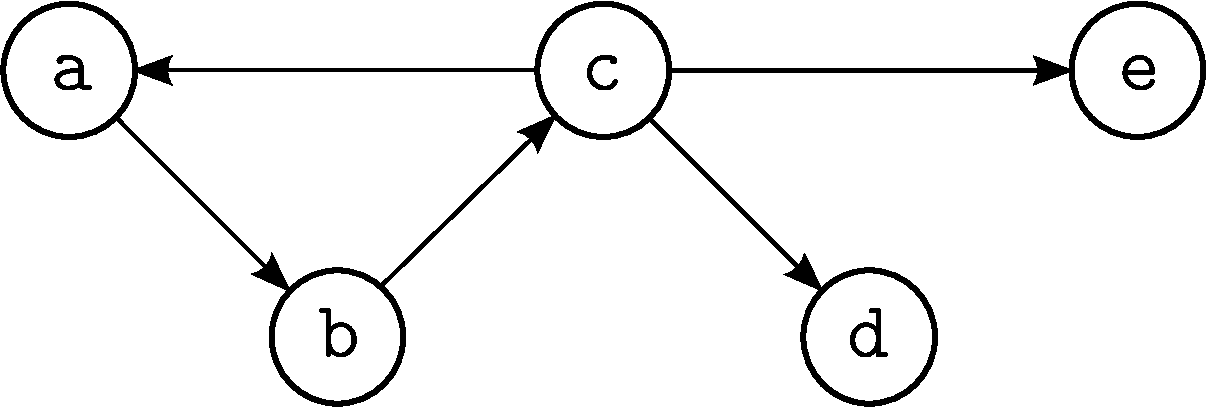
\includegraphics[width=0.5\textwidth]{cdg-loop.pdf}
\end{center}
\caption{带环的有向图}
\label{fig:a_directed_graph_with_a_loop}
\end{figure}

\begin{figure}
\begin{lstlisting}
(define (path node1 node2)
  (bf-path node2 (list (list node1))))

(define (bf-path dest queue)
  (if (null? queue)
      '@
      (let* ((path (car queue))
              (node (car path)))
         (if (eq? node dest)
             (cdr (reverse path))
             (bf-path dest
                      (append (cdr queue)
                              (map (lambda (n)
                                     (cons n path))
                                   (neighbors node))))))))
\end{lstlisting}
\caption{确定性搜索}
\label{fig:deterministic_search}
\end{figure}

从理论上说,非确定性应该可以让我们不用考虑环路带来的问题。
\ref{sec:scheme_implementation} 中给出
的~\emph{choose} 和~\emph{fail} 的深度优先实现是无法解决环路问题
的,但倘若我们当初要求更严格一些的话,那么应该会要求非确定性
的~\emph{choose} 能够依据任意可计算的指标来选择对象,所以这次的例子照
道理也应该不在话下。如果能用上正确版本的~\emph{choose}\index{nondeterministic choice 非确定性选择!correct 正确} 的话,我们就能像图~\ref{fig:nondeterministic_search} 中那样,写出更简短、更清晰的~\texttt{path}。


\begin{figure}
\begin{lstlisting}
(define (path node1 node2)
  (cond ((null? (neighbors node1)) (fail))
        ((memq node2 (neighbors node1)) (list node2))
        (else (let ((n (true-choose (neighbors node1))))
                (cons n (path n node2))))))
\end{lstlisting}
\caption{非确定性搜索}
\label{fig:nondeterministic_search}
\end{figure}

本节会给出一个环路安全的~\emph{choose} 和~\emph{fail} 的实现。
图~\ref{fig:correct_choose_in_scheme} 中真正\index{correct 真正的}的非
确定性~\emph{choose} 和~\emph{fail} 的~Scheme 实现对于环路也能正常
工作。\note{303}只要是等价的非确定性算法能处理的问题,使用了这个版本
的~\emph{choose} 和~\emph{fail} 的程序也一定能找到答案,不过这一点
还会受到硬件的限制。

\begin{figure}
\begin{lstlisting}
(define *paths* ())
(define failsym '@)

(define (true-choose choices)
  (call-with-current-continuation
    (lambda (cc)
      (set! *paths* (append *paths*
                            (map (lambda (choice)
                                   (lambda () (cc choice)))
                                 choices)))
      (fail))))

(define fail)

(call-with-current-continuation
  (lambda (cc)
    (set! fail
          (lambda ()
            (if (null? *paths*)
                (cc failsym)
                (let ((p1 (car *paths*)))
                  (set! *paths* (cdr *paths*))
                  (p1)))))))
\end{lstlisting}
\caption{\emph{choose} 的~Scheme 版正确实现}
\label{fig:correct_choose_in_scheme}
\index{true-choose@\texttt{true-choose}!breadth-first version}
\end{figure}

图~\ref{fig:correct_choose_in_scheme} 中定义的~\texttt{true-choose} 把
用来保存路径的列表当成一个队列来操作。因此,使用~\texttt{true-choose}
的程序对状态空间进行的搜索将是广度优先的\index{nondeterministic choice 非确定性选择!breath-first 广度优先}。每当程序到达选择点的时
候,与每一个选择相对应的续延都会被加入到用来保存路径的列表后
面。(Scheme 的~\texttt{map} 的返回值和~Common Lisp 的~\texttt{mapcar}
的返回值是一样的。) 然后,和之前一样,还是调用~\texttt{fail}。

如果用了这个版本
的~\emph{choose},图~\ref{fig:nondeterministic_search} 里定义
的~\texttt{path} 就能找到一条路径了,事实上,它找到的是最短路径,即
图~\ref{fig:a_directed_graph_with_a_loop} 中所示的
从~\texttt{a} 到~\texttt{e} 的那条路径。

虽然为了内容的完整性,本章给出了正确版本的~\emph{choose}
和~\emph{fail},其实最初的版本就够用了。我们不能仅仅因为其实现不是
形式上正确的,就低估编程语言所提供抽象机制的价值。在用一些语言编程的时
候,感觉上似乎我们能使用任意一个整数,其实能操作的最大一个整数可能只
是~32767。其实只要清楚幻象的限度,那么它所带来的危险就微不足道了,
至少我们的抽象是有保证的。下两章中程序的简洁明了,很大程度上就归功于它
们对非确定性~\emph{choose} 和~\emph{fail} 的善用。

%%% Local Variables:
%%% coding: utf-8
%%% mode: latex
%%% TeX-master: "onlisp-cn"
%%% End:
